%%% ---------------
%%% PREAMBLE
%%% ---------------
\documentclass[11pt,a4paper]{article}

% Define geometry (without using the geometry package)
\usepackage{geometry}
\geometry{landscape, twocolumn, textwidth=27.5cm, textheight=19.5cm, columnsep=15mm}

%\frenchspacing						% better looking spacing

% Call packages we'll need
\usepackage[french]{babel}			% french
\usepackage{graphicx}				% images
\usepackage{amssymb,amsmath}		% math
\usepackage{multicol}				% three-column layout
\usepackage{multirow}
\usepackage{url}					% clickable links
\usepackage{marvosym}				% symbols
\usepackage{wrapfig}				% wrapping text around figures
\usepackage{fontspec}			% font encoding
\usepackage{xunicode}
\usepackage{ragged2e}
\usepackage{titlesec}
\usepackage{framed}
%\usepackage[default]{raleway}
\usepackage{tocvsec2}
% Customize (header and) footer
\usepackage{fancyhdr}
\usepackage{enumitem}
\usepackage{fontawesome}
\usepackage{lipsum}
%\pagestyle{fancy}
\pagestyle{empty}
\setmainfont{Carlito}

%\titlespacing\section{0pt}{0pt plus 4pt minus 2pt}{0pt plus 2pt minus 2pt}
%\titlespacing\subsection{0pt}{12pt plus 4pt minus 2pt}{0pt plus 2pt minus 2pt}
%\titlespacing\subsubsection{0pt}{12pt plus 4pt minus 2pt}{0pt plus 2pt minus 2pt}

%\newfontfamily\headingfont[]{Arial}
%\titleformat*{\section}{\Large\bfseries\sffamily}
%\titleformat*{\section}{\Large\headingfont}

%\renewcommand{\headrulewidth}{0.0pt}	% no bar on top of page
%\renewcommand{\footrulewidth}{0.4pt}	% bar on bottom of page

%%% ---------------
%%% DEFINITIONS
%%% ---------------

% Define separators
\newcommand{\HorRule}[1]{\noindent\rule{\linewidth}{#1}} % Creating a horizontal rule
\newcommand{\SepRule}{\noindent							 % Creating a separator
						\begin{center}
							\rule{250pt}{1pt}
						\end{center}
						}						

% Define Title en News input
\newcommand{\JournalName}[1]{%
		\begin{center}	
			%\Huge \usefont{T1}{augie}{m}{n}
            \Large \usefont{T1}{augie}{m}{n}
			#1%
		\end{center}	
		\par \normalsize \normalfont}
		
\newcommand{\JournalIssue}[1]{%
		\hfill \textsc{\mydate \today, No #1}
		\par \normalsize \normalfont}

\newcommand{\NewsItem}[1]{%
\vspace{3pt}
\underline{\textbf{#1}}
	%	%\usefont{T1}{augie}{m}{n} 	
	%	\large \textbf{#1} %\vspace{3pt}
   %     %\Large #1 \vspace{4pt}
	%	%\par 
   %     \normalsize \normalfont
		  }
		
\newcommand{\NewsAuthor}[1]{%
			\hfill by \textsc{#1} \vspace{4pt}
			\par \normalfont}		

%pas de numérotation des sections
\setsecnumdepth{none}
\setlength{\parindent}{0pt}
%%% ---------------
%%% BEGIN DOCUMENT
%%% ---------------
\begin{document}

\NewsItem{CHANT D'ENTRÉE}
	NOUS SOMMES LE CORPS DU CHRIST,
CHACUN DE NOUS EST UN MEMBRE DE CE CORPS.
CHACUN REÇOIT LA GRÂCE DE L'ESPRIT POUR LE BIEN DU CORPS ENTIER. (bis)
\begin{itemize}
\item[1.]
Dieu nous a tous appelés à tenir la même espérance,
pour former un seul corps baptisé dans l'Esprit.
Dieu nous a tous appelés à la même sainteté,
pour former un seul corps baptisé dans l'Esprit.
\item[3.]
Dieu nous a tous appelés à chanter sa libre louange,
pour former un seul corps baptisé dans l'Esprit.
Dieu nous a tous appelés à l'union avec son Fils,
pour former un seul corps baptisé dans l'Esprit.
\end{itemize}

\NewsItem{PRÉPARATION PÉNITENTIELLE}\\
	Kyrie eleison, Seigneur prends pitié. Kyrie eleison, Seigneur prends pitié.\\
Christe eleison, Ô Christ prends pitié. Christe eleison, Ô Christ prends pitié.\\
Kyrie eleison, Seigneur prends pitié. Kyrie eleison, Seigneur prends pitié.


\NewsItem{GLORIA}
	\begin{itemize}
\item[R/] 
Gloire à Dieu, au plus haut des cieux, et paix sur la terre, aux hommes qu'il aime. (bis)
\item[1.]
Nous te louons, nous te bénissons, nous t’adorons, nous te glorifions, nous   
      te rendons grâce pour ton immense gloire. Seigneur Dieu, Roi du ciel, Dieu 
      le Père tout puissant. R/
\item[2.]
Jésus-Christ, Seigneur Fils unique, Agneau de Dieu, le Fils du Père, toi qui 
      enlèves le péché du monde, reçois nos prières. Toi qui es assis à la droite  
      du Père, prends pitié de nous. R/
\item[3.]
Car toi seul es saint, toi seul es Seigneur, toi seul es le Très Haut : 
      Jésus-Christ, avec le Saint Esprit, dans la gloire de Dieu le Père. R/
\end{itemize}




% -----
\NewsItem{1\iere{} LECTURE} Ac 7, 55-60
% -----

\NewsItem{PSAUME} Ps 96 (97), 1-2b, 6.7c, 9

\textbf{Le Seigneur est roi, le Très-Haut sur toute la terre !}

Le Seigneur est roi ! Exulte la terre !
Joie pour les îles sans nombre !
justice et droit sont l’appui de son trône.

Les cieux ont proclamé sa justice,
et tous les peuples ont vu sa gloire.
À genoux devant lui, tous les dieux !

Tu es, Seigneur, le Très-Haut
sur toute la terre :
tu domines de haut tous les dieux.



% -----
\NewsItem{2\ieme{} LECTURE} Ap 22, 12-14.16-17.20

\NewsItem{ÉVANGILE} Jn 17, 20-26

\NewsItem{HOMÉLIE}

\NewsItem{PROFESSION DE FOI} 

%\newpage

\NewsItem{PRIÈRES UNIVERSELLES} 
Entends nos prières entends nos voix entends nos prières monter vers toi.

\NewsItem{OFFERTOIRE} 

\NewsItem{PRIÈRES SUR LES OFFRANDES}
\textit{Nous nous levons et nous répondons : }
Que le Seigneur reçoive de vos mains ce sacrifice à la louange et à la gloire 
de Son nom, pour notre bien et celui de toute l’Église.

\NewsItem{SANCTUS}
Tu es Saint, Dieu de l'univers, Hosanna au plus haut des cieux. (bis)      
Le ciel et la terre sont remplis de ta gloire. 
Béni soit celui qui vient au nom du Seigneur.


%\begin{itemize}
%\item[R/] Trois fois Saint, trois fois Saint, le Seigneur Dieu de l’univers. 
%      Hosanna, hosanna (bis) au plus haut des Cieux ! 
%\item[1.]  Le Ciel et la Terre nous chantent Ta gloire, hosanna au plus haut des Cieux. 
%      Béni soit Celui qui vient, c’est Jésus notre Sauveur ! 
%\end{itemize}

\NewsItem{ANAMNÈSE}
Gloire à toi qui étais mort, gloire à toi qui es vivant,
notre Sauveur et notre Dieu. Viens Seigneur Jésus.


\NewsItem{NOTRE PÈRE}

\NewsItem{AGNUS}

Agneau de Dieu qui enlèves le péché du monde, prends pitié de nous (bis)\\
Agneau de Dieu qui enlèves le péché du monde, donne-nous la paix

\NewsItem{COMMUNION}
\textbf{Venez approchons}
\begin{itemize}
\item[R.]
Venez ! Approchons-nous de la table du Christ,
Il nous livre son corps et son sang,
Il se fait nourriture, Pain de Vie éternelle,
Nous fait boire à la coupe des Noces de l’Agneau !
\item[1.]
La Sagesse de Dieu a préparé son vin,
Elle a dressé la table, elle invite les saints :
\og Venez boire à la coupe ! Venez manger le pain !
Soyez la joie de Dieu, accourez au festin ! \fg
\item[2.]
Par le pain et le vin reçus en communion,
Voici le sacrifice qui nous rend à la Vie.
Le sang de l’Alliance jaillit du cœur de Dieu,
Quand le Verbe fait chair s’offre à nous sur la Croix.
\item[3.]
Dieu est notre berger, nous ne manquons de rien,
Sur des prés d’herbe fraîche, Il nous fait reposer.
Il restaure notre âme, Il nous garde du mal,
Quand Il dresse pour nous la Table du Salut.
\end{itemize}


\NewsItem{CHANT D'ENVOI}
Esprit de lumière, Esprit créateur
\begin{itemize}
\item[1.]
Viens, Esprit du Dieu vivant,
Renouvelle tes enfants,
Viens, Esprit Saint, nous brûler de ton feu !
Dans nos cœurs, répands tes dons,
Sur nos lèvres, inspire un chant,
Viens, Esprit Saint, viens transformer nos vies !
\item[R.]
Esprit de lumière, Esprit créateur,
Restaure en nous la joie, le feu, l’espérance.
Affermis nos âmes, ranime nos cœurs,
Pour témoigner de ton amour immense.
\item[2.]
Fortifie nos corps blessés,
Lave-nous de tout péché,
Viens, Esprit Saint, nous brûler de ton feu !
Fais-nous rechercher la paix,
Désirer la sainteté,
Viens, Esprit Saint, viens transformer nos vies !
\end{itemize}


\newpage


\NewsItem{Intentions de messe (Sainte Croix)}
\begin{itemize}
\item[\Cross]
Marie Jeanne et Fernand FONTAINE.
\item[\Cross]
Winckel Marianne et Caroline BERG
\end{itemize}

\NewsItem{Informations paroissiales}

%\begin{framed}
\begin{tabular} {lcp{8cm}}
\multicolumn{3}{c}{\textbf{Saint Jean-Baptiste} } \\ \hline
Mardi    & 03 juin : & Vêpres 18h15. Messe 18h30 \\ \hline
Jeudi    & 05 juin : & 
Exposition du Saint Sacrement à 16h00. Adoration. Salut au Saint Sacrement à 18h15. Messe à 18h30 
 \\ \hline
Vendredi & 06 juin : & Laudes 08h45. Messe 09h00 \\ \hline
Samedi   & 07 juin : & Messe anticipée 18h00 \\ \hline
Dimanche & 08 juin : & \emph{Pentecôte} \textit{Profession de foi} Messe 10h00 \\ \hline
\multicolumn{3}{c}{\textbf{Sainte Croix} } \\ \hline
Mercredi & 04 juin : & Messe 09h00 \\ \hline
Dimanche & 08 juin : & pas de messe \\ \hline
\multicolumn{3}{c}{\textbf{Résidence Landsberg (3 rue Jean Monnet)} } \\ \hline
Mercredi & 04 juin : & Messe 10h45 \\ \hline
\end{tabular}

\begin{framed}
\begin{tabular} {lcp{8cm}}
\multicolumn{3}{c}{\textbf{Saint Jean-Baptiste} } \\
Dimanche & 01 juin : & 16h00 Concert Spirituel avec Véronique REINBOLD-WENDLING et Estelle GERTHOFFERT (orgue). Entrée libre. Plateau.
\end{tabular}
\end{framed}
%\end{framed}


\NewsItem{Répétitions des chorales}
\begin{description}
\item[Chorales paroissiales] : vendredi 20h15 à Sainte Croix
\end{description}

\begin{framed}
\textbf{Presbytère St Jean-Baptiste}
%2 rue de l'école 67380 Lingolsheim 03 88 78 16 45 \\
2 rue de l'école 67380 Lingolsheim \phonenumber[country=FR]{0388781645} \\
\textbf{Permanence} Lun. au Jeu. : 09h30-12h00 et 15h-18h. Ven. 16h-18h00. Sam. 09h30-12h00. \\
\textbf{Courriels} \texttt{nddessables@hotmail.com}, \texttt{danielette67380@gmail.com}

%\textbf{Caritas} Vestiaire ouvert le mardi de 14h à 16h

\texttt{https://stjeanbaptistelingo.fr} \hfill \faFacebook Catho Lingo \hfill \faInstagram @catho\_lingo
\end{framed}



%         \begin{tabular}{l l l}
%         \multicolumn{3}{c}{\textbf{St Jean-Baptiste}} \\
%  Mardi & 11 fév. & Vêpres 18h15 - 18h30. Pas de messe \\
%Jeudi & 13 fév. & Salut au Saint Sacrement 18h15. Messe 18h30. \\
%    Vendredi & 14 fév. & Laudes 08h45 - 09h00. Pas de messe \\
%        Samedi  & 15 fév. & Messe anticipée 18h00 \\
%    Dimanche & 16 fév. & Pas de messe \\      
%      
%         \multicolumn{3}{c}{\textbf{Ste Croix}} \\
%         Mercredi & 12 fév. & Pas de messe \\ 
%         Dimanche & 16 fév.& Messe 10h30 \\
%    
%        \end{tabular}
  

\newpage

\JournalName{Communauté de Paroisses de Lingolsheim \\
\normalsize \textit{Notre Dame des Sables}
\\ \large \'{E}glise Saint Jean-Baptiste
\\  \normalsize \textit{7\ieme{} Dimanche de Pâques - Année C}
\\ \large Dimanche 01 juin  2025}
%\noindent\HorRule{3pt} \\[-0.75\baselineskip]
%\HorRule{1pt}
% -----

% Front article
% -----
%\vspace{0.5cm}
%	\SepRule
%\vspace{0.5cm}

%\begin{center}
\begin{minipage}[h]{1.0\linewidth}
 \begin{center}
 \textbf{
 %\dots
\og 
Rentrée Pastorale 2025-2026
 \fg{}
 %\dots
 }
 \end{center}

%\begin{wrapfigure}{l}{1.3cm}
%\vspace{-0.4cm}
%	\includegraphics[scale=1.0]{../images/lazarre}
%\end{wrapfigure}
Une nouvelle rentrée pastorale qui nous réjouit tous. En effet, après un temps de répit, il nous revient de mettre en marche la machine de nos activités pastorales.

Au début de cette nouvelle année pastorale, je souhaite vous redire toute ma joie de vous retrouver pour continuer la mission qui m’est assignée dans notre communauté de paroisses. Et comme chaque année, nous mettrons l’accent en premier lieu sur la vie catéchétique des enfants et des adolescences, l’animation liturgique, la création d’une troisième chorale, la visite aux malades et dans notre maison de retraite ( \emph{Résidence du Parc}), l’accueil et l’accompagnement en vue de baptêmes,  du catéchuménat des adultes, des mariages, l’encadrement  des servants d’autel, l’entretien de notre église pour la rendre  accueillante, avec ces innombrables petits gestes de service qui jalonnent l’existence ; tout cela nous aidera à vivre une véritable dimension ecclésiale.

Je voudrais vous remercier de tout cœur, vous tous qui êtes des membres vivants et actifs de la communauté paroissiale que nous formons, véritable artisans de l’évangélisation ordinaire. Mon souhait pour la vie de notre communauté de paroisses est que nous arrivions toujours plus à nous ouvrir et à nous connaître les uns les autres, à nous apprécier dans ce que nous sommes et vivons.

L’année dernière, avec toutes les entités de nos deux paroisses, nous avons eu différentes propositions, activités et invitations qui ont favorisées l’\textbf{Unité et l’ouverture} qui constituaient notre thème pastoral. Ne manquons pas cette année ces moments simples et conviviaux qui permettent de tisser des liens gratuits, profonds et tout simplement chrétiens.

\begin{wrapfigure}{l}{1.2cm}
\vspace{-0.4cm}
	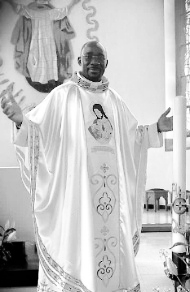
\includegraphics[scale=1.20]{../images/standing_daniel}
\end{wrapfigure}
Cette année nous porterons ensemble cette rentrée dans le cœur de chacun avec nos \textbf{jeunes pro}. Chacun à son rythme, selon ses possibilités et ses réalités mais avec un seul et même objectif : l’accomplissement de nos activités communautaires. Présentons également notre rentrée paroissiale au Christ. Et continuons notre chemin pour la mise en œuvre de notre projet paroissial autour de ce principal thème : \textbf{\og Avec notre jeunesse bâtissons une communauté plus dynamique, rayonnante et missionnaire\fg{}.}

	Que cette rentrée pastorale nous aide à prendre des résolutions nécessairement pour plonger à frais nouveaux dans la parole et être des disciples crédibles de l’évangile.


\begin{flushright}
Bonne rentrée pastorale à toutes et à tous !
\textit{Père  Daniel  ETTÉ}
\end{flushright}


%\lipsum[1-3]
\end{minipage}
%\end{center}
% -----
\end{document} 
